% !TeX encoding = utf8
% !TeX spellcheck = fr

\chapter{Atmosphère et instruments}\label{cha:atmosph}

\begin{framed}
	\begin{center}
		\xc{} est entièrement développé par des bénévoles.\\
		Cette documentation aussi.\\
		Si vous y voyez des imperfections, vous pouvez facilement les faire disparaître~:\\
		\xcsoarwebsite{/develop/}
	\end{center}
\end{framed}

\xc{} comporte un modèle interne de l'atmosphère basé sur les statistiques collectées lors du vol et par les périphériques connectés.
Ces statistiques et ses mesures sont approximatives et la météo peut changer rapidement certains jours.
Le pilote doit observer en permanence la météo.
En particulier, lors d'une vache, le pilote doit rechercher les indications au sol pour confirmer la force et la vitesse du vent.

\section{Variomètre}\label{sec:variometer}

Un affichage de style cadran à aiguille montre les valeurs du variomètre.
Les valeurs brutes du variomètre contrôlent la flèche principale du cadran, et, dans le centre du cadran, la valeur brute est affichée sous forme de chiffres.

De plus, les flèches de vitesse optimale (chevrons) sont au-dessus ou en dessous les valeurs du variomètre.
Des chevrons pointant vers le haut recommandent de ralentir.
Des chevrons pointant vers le bas recommandent d'accélérer.

Quand la valeur moyennée est affichée, la valeur affichée est la vitesse verticale moyenne sur les 30~dernières secondes si l'on est en mode Spirale, et la vitesse verticale nette (de la masse d'air) sur les 30~dernières secondes si l'on est en mode Transition.

\marginpar{\includegraphics[angle=0,width=0.5\linewidth,keepaspectratio='true']{figures/gaugevario2.png}}

La valeur moyenne peut aussi être affichée comme une aiguille supplémentaire additionnelle (curseur).
Le cadran du variomètre est configurable \config{variogauge}, en particulier les informations à afficher en plus du variomètre brut.

Quand un variomètre intelligent est connecté à \xc, l'aiguille affiche les données produites par l'instrument.
Sinon, il fournit des valeurs estimées sur la base de la vitesse verticale du GPS, qui a du retard et n'est pas compensé en énergie totale.

Les valeurs du MacCready, des moucherons, des ballast, de la vitesse optimale et des données du vent sont transférées entre \xc{} et les variomètres intelligents externes supportés.
Dans une configuration idéale, à la fois \xc{} et le variomètre partagent une vue cohérente du vol à tout instant. Ainsi, en ajustant le calage MacCready sur l'un des instruments, il devrait être gardé synchrone sur le second par l'intermédiaire du logiciel, et ne pas demander de saisie particulière de la part du pilote.

Des pilotes sur-utilisent la synchronisation des périphériques (voir section~\ref{conf:comdevices}) pour différentes raisons.
Vous pourriez avoir des calages MacCready différents dans \xc{} et un variomètre intelligent pour vérifier les résultats.
Vous pourriez faire des calculs avec différentes configurations des ballasts pour vérifier les résultats
Vous pourriez sélectionner manuellement sur l'un des instruments des paramètres de vent différents pour vérifier les résultats, etc.

Une liste des variomètres supportés est disponibles dans la section~\ref{sec:supported-varios}.

Pour le Vega~: un petit icône représentant un planeur en spirale est affiché quand le variomètre est en mode Spirale audio.

\section{Variomètre sonore}

En plus de l'affichage du variomètre, \xc{} fournit un variomètre acoustique qui convertit les valeurs du variomètre en sons. Le variomètre sonore est pour l'instant uniquement disponible pour les appareils sous Android.
Pour de bonnes performances, connectez à votre appareil un capteur barométrique ou utilisez celui de votre appareil Android s'il en dispose. 
Le variomètre sonore peut être activé/désactivé dans la configuration des jauges.


\section{Informations additionnelles}

Quand des informations additionnelles sur la dynamique du planeur ou sur la masse d'air sont fournis par un variomètre intelligent, \xc{} est souvent capable de les utiliser ou de les afficher dans une InfoBoxe séparée. 

Les valeurs des capteurs clefs que \xc{} utilise incluent~:
\begin{description}
\item[Variometre brut à énergie totale] (taux de changement de l'énergie totale du planeur) Utilisé pour l'affichage, et pour le calcul du variomètre netto.
\item[Variomètre Netto] (vitesse verticale estimée de la masse d'air autour du planeur) Utilisé pour l'affichage, et pour colorer la trace de cheminement de façon à montrer les zones d'ascendances et de descendances.
\item[Accélération du planeur] (facteur de charge) Utilisé pour les calculs du vario netto quand un variomètre externe netto n'est pas disponible.
\item[Altitude barométrique] Utilisé pour l'affichage.
\item[Vitesse indiquée] Utilisé pour l'affichage, dans les calculs de compensation en arrivée pour l'énergie cinétique, et pour les calculs de variomètre netto quand un variomètre netto externe n'est pas disponible.
\item[Densité de l'air] Utilisé pour calculer la vitesse air réelle à partir de la vitesse indiquée.
\end{description}

\section{Affichage du vent}

Un affichage continu de la force et de la direction du vent est donné sur la carte.
L'information sur le vent provient de la dérive du planeur sous l'effet du vent pendant les spirales (mode Thermique).

La vitesse et la direction du vent sons affichés comme un vecteur de vent sur la carte mobile et optionnellement sous forme numérique dans les champs d'affichage des données.
La longueur du vecteur indiquant la vitesse du vent, et cette vitesse est aussi affichée à proximité du vecteur de vent.

Les données sur le vent est l'une des nombreuses sources de données utilisées pour le calcul des informations sur l'arrivée.
Il est possible de modifier manuellement le vent utilisé dans ces calculs.

\begin{center}
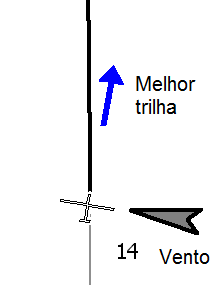
\includegraphics[angle=0,width=0.4\linewidth,keepaspectratio='true']{figures/optwind.png}

%TODO{\it DIAGRAM CUTOUT SHOWING WIND VECTOR AT GLIDER, MAYBE ALSO SHOW A
%WINDSOCK NEXT TO THE DISPLAY TO MAKE THE DIRECTION OBVIOUS.  NO
%TERRAIN/TOPOGRAPHY}

\end{center}

\section{Estimation du vent}\label{sec:wind-estimation}

\xc{} permet d'estimer le vent au cours du vol de deux manières~:
\begin{description}
\item[Spirale] Cette méthode utilise les positions GPS pour estimer le vent sur la base de la dérive, typiquement lors d'une spirale.
Elle est disponible dans toutes les installations d'\xc.
\item[Zigzag] Cette méthode utilise les positions GPS et les mesures de vitesse air vraie pour estimer le vent, typiquement lors d'une transition.
Elle est uniquement disponible quand \xc{} est connecté à un variomètre intelligent qui fournit une vitesse air vraie.
\end{description}

La vitesse et la direction du vent peuvent aussi être ajustées manuellement dans la fenêtre de paramétrage du vent (voir ci-dessous).

Les statistiques sont collectées de façon à enregistrer les vents à différentes altitudes et moments.
Quand l'altitude du planeur change significativement, les statistiques sont consultées pour déterminer la meilleure estimation du vent sur la base des mesures précédentes.

Pour les PC avec un écran tactile, vous pouvez aussi le faire en surlignant l'InfoBoxe du vent et en utilisant les flèches du curseur (Haut et Bas pour augmenter et diminuer la vitesse, Gauche et Droite pour faire tourner la direction du vent).

Les paramètres de configuration \config{autowind} permet de contrôler quelle méthode d'estimation est utilisée pour les mises à jour du vent, grâce au champ `Vent Auto'~:
\begin{itemize}
\item Manuel
\item Spirale
\item Zigzag
\item Les deux (Zigzag et Spirale)
\end{itemize}

Quand le vent estimé change significativement, une notification par message d'état spécifique est affichée.

\subsection*{Algorithme du vent en spirale}

\xc{} estime la vitesse et la direction du vent lors des spirales.
C'est effectué en utilisant un algorithme sophistiqué qui améliore par incrément le vent estimé à partir des virages terminés.
Les virages de pauvre qualité, où l'inclinaison change significativement, sont rejetés ou ont un impact mineure sur l'estimation globale du vent.
Les meilleurs virages sont ceux ayant une inclinaison constante.
Les estimations sont obtenues uniquement si, en moyenne, au moins une position GPS est effectuée toutes les deux secondes.
Cela conduit à améliorer la qualité des estimations quand il y a des positions GPS déclassées.

%TODO{\it DIAGRAM SHOWING WIND CALCULATION, BAD TURN AND GOOD TURN}

\subsection*{Algorithme Zigzag}

Pour les planeurs disposant d'un variomètre intelligent connecté à \xc, un algorithme d'estimation du vent appelé ``zigzag'' est disponible.
Avec cet algorithme, l'estimation du vent peut être mise à jour en continu au cours de long vol sans spirale.

Cela permet de mettre à jour l'estimation du vent au cours des transitions quand le planeur effectue des manœuvre en zigzag.
Aucune manœuvre spécifique n'est nécessaire, car dans beaucoup de cas l'estimation sera mise à jour lorsque le cap de l'avion sera modifiée par le pilote en recherche d'ascendance.
En général, l'algorithme nécessite que le cap du planeur change de plus de 40°.

Si le vent change significativement pendant un vol en ligne droite, l'algorithme zigzag est utilisé pour mettre à jour le vent estimé même si le cap du planeur ne change pas beaucoup.
Cela fournit une plus grande précision lors des longues arrivées.

Les estimations du vent sont mises à jour quand une grande différence entre la vitesse sol estimée et la vitesse sol réelle sont détectées même avec peu de manœuvres en zigzag.

\subsection*{Algorithme avec compas}

Pour les planeurs avec un variomètre intelligent et un compas numérique connectés à \xc, un algorithme d'estimation du vent et de la vitesse air est en développement.
Cela fournit une autre méthode de mise à jour de l'estimation du vent au cours des transitions et ne nécessite pas de manœuvres en zigzag.

\section{Fenêtre de paramétrage du vent}\label{sec:wind-setup}

La fenêtre de paramétrage du vent permet de fournir une première estimation de la vitesse et de la direction du vent, en général avant le vol.
\menulabel{\bmenug{Config 1}\blink\bmenug{Vent}}

\begin{center}
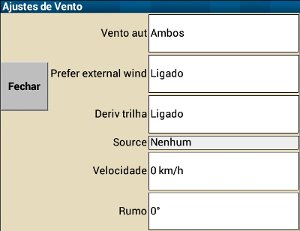
\includegraphics[angle=0,width=0.4\linewidth,keepaspectratio='true']{figures/dialog-wind2.png}
\end{center}

À n'importe quel moment au cours du vol, le pilote peut apporter des corrections à l'estimation du vent en entrant des corrections dans la fenêtre de paramétrage du vent.
Une fois la fenêtre fermée, l'estimation interne est ignorée jusqu'à ce qu'une nouvelle estimation interne soit obtenu par les algorithmes de spirale ou zigzag.

L'algorithme d'estimation automatique du vent peut aussi être activé/désactivé ou être changé de mode dans cette fenêtre.
Voir section~\ref{sec:wind-estimation} pour des détails sur ces algorithmes.

La compensation de la dérive due au vent sur la trace de cheminement peut aussi être activée/désactivée dans cette fenêtre.
Voir section~\ref{sec:trail} pour des détails sur les conséquences en terme d'affichage de la trace de cheminement.

\section{Profil d'ascendance}

Les statistiques sur les taux de montée en ascendance sont collectés et affichés dans le profil des ascendances.
Ce profil est affiché au-dessus de la barre des différences de hauteur au plan d'arrivée, sur la gauche de la carte.
Il n'est pas affiché quand le planeur est au-dessus du plan d'arrivée.

Le profil des ascendances montre un graphique où l'axe vertical part de la hauteur au-dessus de la hauteur de garde au sol (section~\ref{sec:safety-heights}), et est mis à l'échelle jusqu'à la hauteur maximale atteinte.
L'axe horizontal est le taux moyen de montée atteint pour une gamme d'altitude donnée.
L'échelle de l'axe horizontal dépend du calage MacCready, une flèche indiquant cette valeur.
L'altitude présente du planeur est surimposée dans une zone ombrée.
Cette échelle et la flèche permettent au pilote de comparer rapidement son calage MacCready et au taux de montée dans les ascendances, et ainsi de choisir sa gamme d'altitude de travail.

\marginpar{\hbox{\vbox{\includegraphics[angle=0,width=0.7\linewidth,keepaspectratio='true']{figures/thermalprofile.png}}}}

En transition entre des ascendances, la position verticale de la flèche, qui indique la hauteur de planeur dans le profil des ascendances, peut être utilisée comme référence afin de réfléchir sur l'urgence à trouver une nouvelle ascendance.

Quand la flèche se rapproche de la base du profil, le planeur se rapproche de la garde au sol et le pilote doit considérer prendre même une faible ascendance.

\section{Repère des ascendances}
Un algorithme évalue la position du centre des ascendances lors des spirales.
Le symbole du repère des ascendances est un cercle vert avec une spirale.

\begin{center}
\includegraphics[angle=0,width=0.8\linewidth,keepaspectratio='true']{figures/shot-tlocator-circling.png}
\end{center}

Le repère des ascendances marque la position des 20~dernières ascendances sur la carte avec le symbole d'ascendance au cours des transitions.

La position est calculée pour compenser le décalage de l'ascendance en fonction de l'altitude du planeur.
Cela signifie, qu'en interne, \xc{} mémorise la position au sol de la source de l'ascendance.
Autrement dit, si vous quittez une ascendance à son sommet et y revenait à une altitude inférieure, la position sur la carte donne la position prédite de l'ascendance à votre altitude plus inférieure (qui est décalée au vent par rapport au sommet).

Si le vent change et que la source de l'ascendance est toujours active, sa position sur la carte prend en compte le changement de vent~; c.-à-d.\ que l'ascendance en altitude est projetée sous le vent du nouveau vent estimé.

\begin{center}
\includegraphics[angle=0,width=0.8\linewidth,keepaspectratio='true']{figures/shot-tlocator-cruise.png}
\end{center}


\section{Assistant thermique}\label{sec:thermal-assistant}

L'assistant thermique est une aide graphique pour maximiser l'exploitation d'une ascendance donnée.
S'il est activé, \config{thermalassistant} un petit diagramme polaire est affiché dans le coin inférieur gauche de l'écran. Un simple pression sur le petit diagramme le fait passer en vue plein écran.

Le diagramme polaire montre le taux de montée sur le trajet circulaire du planeur.
Les copies d'écran montre une spirale à droite où le planeur est positionné sur le coté gauche.
La distribution polaire du taux de montée est affiché par rapport à la position présente du planeur.


\begin{tabular}{c c}
\includegraphics[angle=0,width=0.5\linewidth,keepaspectratio='true']{figures/dialog-thermal-assistant0.png}&
\includegraphics[angle=0,width=0.5\linewidth,keepaspectratio='true']{figures/dialog-thermal-assistant1.png}\\
\end{tabular}

Les deux copies d'écran sont prises à quelques secondes d'intervalle pour montrer l'utilisation pratique du diagramme de taux de montée pivotant.
Une façon simple d'optimiser le taux de montée en se basant sur l'assistant est de suivre de manière répétitive les deux étapes suivantes~:
\begin{description}
\item[1.]  Au moment où le taux maximum de montée sur le diagramme polaire passe par le haut du graphique, c.-à-d.\ un quart de tour avant que vous n'atteignez ce point, ouvrez un peu la spirale pour déplacer le centre de la spirale dans la direction du taux de montée maximum.
\item[2.]  Au moment où le taux maximum de montée sur le diagramme polaire passe par la position du planeur, c.-à-d.\ lorsque le vario doit être à son maximum, refermez la spirale pour vous centrer sur le maximum de l'ascendance.
\end{description}

On doit se rappeler que l'interprétation de l'assistant thermique se base toujours sur le delai particulier du capteur connecté ou de l'appareil lui-même.
Une bonne optimisation de la montée demandera ainsi un peu de d'habitude afin de prendre en compte ce délai.


\section{Prévision de la convection}\label{sec:convection-forecast}

Si le planeur est équipé avec une sonde de température et d'humidité extérieures, un système simple de prévision de la convection estime le plafond de la convection et la base des nuages.
La sonde d'humidité est optionnelle et est principalement utilisée pour l'estimation de la base des nuages.

Avant le décollage ou au cours du vol, le pilote peut modifier la température maximale prévue au sol en ajustant la valeur dans l'InfoBoxe ``Température prévue''.

Le plafond de convection prévu est déterminé par l'altitude à laquelle la température atmosphérique est égale à la température maximale prévue au sol, diminuée selon l'adiabatique sèche. %TODO Translation to be improved
Généralement, le planeur n'atteindra pas le plafond de convection, aussi, les valeurs mesurées sont extrapolées pour estimer le plafond.
Si l'atmosphère est stable, l'altitude du plafond de convection est donnée comme nulle.

La température maximale prévue au sol est entrée en utilisant la fenêtre des paramètres de vol décrit en section~\ref{sec:flight-setup}.


%TODO{\it DIAGRAM SHOWING THERMAL FORECAST, STABLE WITH CLOUD}
%
%TODO{\it DIAGRAM SHOWING THERMAL FORECAST, UNSTABLE }

La base des nuages prévue est déterminée par l'altitude à laquelle le point de condensation croise la température maximale prévue au sol, diminuée selon l'adiabatique sèche. %TODO Translation to be improved
Si aucun nuage n'est prévue, l'altitude de base des nuages est donnée comme nulle.


%TODO{\it DIAGRAM SHOWING THERMAL FORECAST, STABLE WITH NO CLOUDS}

\section{Fenêtre d'analyse}

La fenêtre d'analyse est utilisé pour visualiser différents aspects de l'atmosphère.
\menulabel{\bmenug{Info 1}\blink\bmenug{Analyse}}

Les différentes pages sont~:
\begin{description}

\item[Vent en altitude]
Montre un graphique de la vitesse du vent en fonction de l'altitude, ainsi que les vecteurs du vent à différentes altitudes.

Le bouton `Régl.\ vent' ouvre le fenêtre de paramétrage du vent (par ex.\ pour ajuster manuellement le vent).

\begin{center}
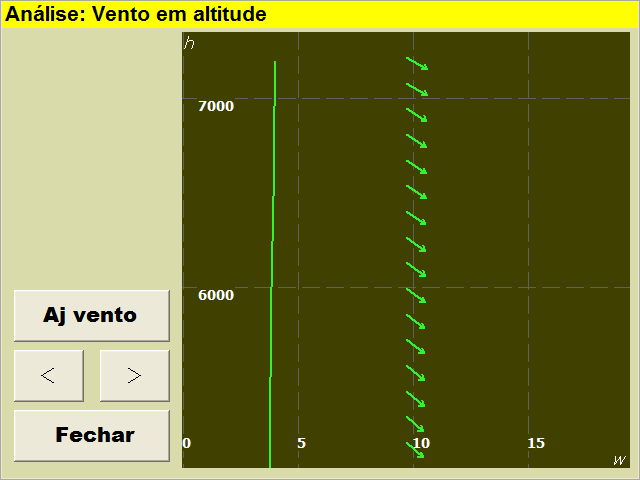
\includegraphics[angle=0,width=0.8\linewidth,keepaspectratio='true']{figures/analysis-wind.png}
\end{center}

\item[Profil de température]
Cette page est disponible uniquement si un instrument supporté est connecté à \xc{} et fournit la température et l'humidité de l'air extérieur.
Le graphique montre la variation de la température d'air sec, la température du point de condensation et la température de l'air extérieur avec l'altitude.
La prévision de la convection est résumée en une altitude estimée de convection thermique et une base des nuage estimée.

\begin{center}
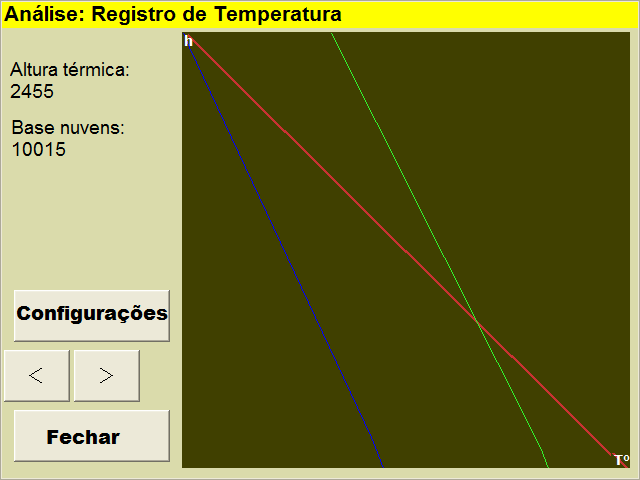
\includegraphics[angle=0,width=0.8\linewidth,keepaspectratio='true']{figures/analysis-temptrace.png}
\end{center}

\end{description}
Les pages d'historique des ascendances et du barographe, décrit en section~\ref{sec:analysis-climb}, sont elles-aussi utiles pour déterminer les tendances des conditions de vol à voile.

\section{Météo, METAR / TAF}\label{sec:metar-taf}

Si le matériel sur lequel tourne \xc{} peut se connecté à Internet, des rapports météo et des prévisions peuvent être téléchargés.
\menulabelr{\bmenug{Info}\blink\bmenug{Météo}}
Les informations disponibles en temps réel sont signalées par un petit drapeau attaché au point de virage de la station météo.
Pour paramétrer les rapports et les prévisions, ouvrez la fenêtre `METAR et TAF'.
\menulabelr{\includegraphics[width=0.6cm]{icons/map_weather_station.pdf}}
En faisant \bmenuw{Ajouter}, un écran de filtres des codes ICAO s'affiche.
Après avoir entré le nom et appuyé sur \bmenuw{OK}, une nouvelle station est ajoutée à la liste.
Accéder à l'information est possible soit en sélectionnant un aéroport et en appuyant sur \bmenuw{Détails} sur le même écran, soit en appuyant sur la carte et en sélectionnant la fenêtre ``Éléments de la carte à cet endroit''.
La fenêtre affichera les aéroports, les espaces aériens\textellipsis et les données météo.
Si les drapeaux ne s'affichent pas sur la carte, c'est qu'aucune information n'est actuellement disponible.
Ouvrez la fenêtre d'infomation et appuyez sur \bmenuw{Mettre à jour}.

\section{Prévisions météo, RASP}\label{sec:weather-forecast}

Le ``Regional Atmospheric Soaring Prediction'' (ou RASP --- pour ``prédiction atmosphérique régionale vélivole'') vise à fournir des prévisions météo graphiques détaillées pour des objectifs de vol à voile.
Plus plus de détails, le pilote intéressé est invité à consulter \url{http://www.drjack.info} sur le fonctionnement des prévisions RASP, sur leurs disponibilités géographiques, leurs utilisations et leurs limites.
\url{http://www.drjack.info/RASP} fournit une liste des zones couvertes par des prévisions RASP, prévisions diffusées par de nombreux bénévoles vélivoles et parapentistes.
Notez que certains liens ne fournissent des données que pendant la saison favorable et que seulement une partie diffuse des données au format \xc{}.

Pour être utilisé dans \xc, un fichier \verb|xcsoar-rasp.dat| doit être installé dans le répertoire XCSoarData.
En février 2014, le téléchargement des fichiers \verb|xcsoar.rasp.dat| n'est pas (encore) supporté par le gestionnaire de fichiers d'\xc.
Les prévisions RASP sont affichées comme des surcouches de couleur sur la carte de relief.\\ \\
Assurez-vous que l'affichage du relief soit activé. \tip{} \\ \\

Les surcouches de prévision RASP sont activables par le menu
\menulabelr{\bmenug{Info}\blink\bmenug{Météo}}
\bmenug{Info}.

Le paramètre Champ détermine le type de donnée à afficher sur le carte.
Le paramètre Temps détermine l'heure de la prévision affichée sur la carte. 
Une fois les paramètres météo rentrés, le paramètre de temps sera mis à jour au moment le plus proche disponible dans le fichier RASP.\@
Quand un champ n'est pas disponible dans une fichier RASP, son arrière-plan est vide.

Les valeurs maximales et minimales du type de données apparaissant sur la carte sont dessinées 
\marginpar{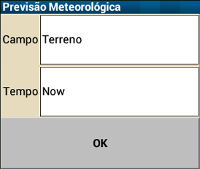
\includegraphics[angle=0,width=0.95\linewidth,keepaspectratio='true']{figures/dialog-weather.png}}
à leurs localisations respectives.
Le type de données est affiché dans le coin inférieur gauche de l'écran.

Les types de données disponibles pour affichage sont~:
\begin{description}
\item[Relief] Affiche le relief sur la carte, aucune donnée météo n'est affichée.

\item[W*] 
Force moyenne des ascendances thermiques en air sec à mi-hauteur de la couche convective.
Soustrayez le taux de chute du planeur pour estimer le vario moyen pour des thermiques sans nuage.
La force des ascendances sera supérieure à celle prévue si des nuages convectifs sont présents, puisque la condensation des nuages améliore la flottabilité de l'air (c.-à-d.\ que la prédiction néglige la ``succion nuageuse''). %TODO translation to be improved
Cette valeur dépend à la fois du réchauffement du sol et de l'épaisseur de la couche limite.

\begin{center}
\includegraphics[angle=0,width=0.8\linewidth,keepaspectratio='true']{figures/rasp-wstar.png}
\end{center}

\item[BL wind spd]
La vitesse et la direction du vecteur moyen du vent dans la couche-limite.
Cette prédiction peut être trompeuse s'il y a un fort changement de direction du vent dans la couche limite.

\begin{center}
\includegraphics[angle=0,width=0.8\linewidth,keepaspectratio='true']{figures/rasp-blwindspd.png}
\end{center}

\item[H bl]  
Altitude du sommet de la couche de mélange qui, pour la convection thermique, est le sommet moyen des thermiques sec.
Au-dessus d'un relief plat, les hauteurs maximales des ascendances seront plus faibles à cause du taux de chute du planeur et d'autres facteurs.
En présence de nuages (qui améliore la flottabilité de l'air, créant une ``succion nuageuse''), le sommet des ascendances sera plus haut que prévu, mais la hauteur maximale d'exploitation des ascendances sera limitée par la base des nuages.
De plus, quand le mélange est causé par des turbulences cisaillantes plutôt que par de la convection thermique, ce paramètre ne sera pas utile pour les vols en planeur.

\begin{center}
\includegraphics[angle=0,width=0.8\linewidth,keepaspectratio='true']{figures/rasp-hbl.png}
\end{center}

\item[dwcrit]
Ce paramètre estime la hauteur au-dessus du sol à laquelle la force moyenne des thermiques secs passe en-dessous de 1,1~m/s (225~pieds/min.).
Il est attendu qu'il donne de meilleures estimations quantitatives de la hauteur maximale des thermiques sans nuage que l'altitude du sommet de la couche limite, en particulier quand le mélange provient plus d'un cisaillement vertical du vent que de thermiques.
(Note~: les hypothèses actuelles tendent à sous-estimer la hauteur maximale de convection en conditions sèches)
En présence de nuages, la hauteur maximale d'exploitation des thermiques pourrait être limitée par la base des nuages.
Étant pour des thermiques ``secs'', ce paramètre ne prend pas en compte l'effet de ``succion nuageuse''.

\item[hwcrit]  
Similaire à \emph{dwcrit}, mais pour une altitude au lieu d'une hauteur.

\item[bl cloud]
Ce paramètre fournit un moyen supplémentaire d'évaluer la formation des nuages dans la couche limite et pourrait être utilisé soit en conjonction avec les autres paramètres de prévision nuageuse, soit à leur place.
Il suppose une relation très simple entre le pourcentage de couverture nuageuse et l'humidité relative maximale au sein de la couche limite.
L'altitude de la base des nuages n'est pas prédite, mais on s'attend à ce qu'elle soit inférieure à l'altitude du sommet de la couche limite.

\begin{center}
\includegraphics[angle=0,width=0.8\linewidth,keepaspectratio='true']{figures/rasp-blcloudpct.png}
\end{center}

\item[Sfc temp] 
La température à 2~m au-dessus du sol.
Elle peut être comparée aux températures de surface observées afin d'avoir une indication sur la qualité des prévisions du modèle~; par ex.\ si les températures observées au sol sont significativement plus faibles que celles de la prévision, les conditions de vol à voile seront moins intéressantes que prévues.
\item[wblmaxmin]
Mouvement vertical maximum, moyenné sur la surface du maillage, au sein de la couche limite créée par la convergence horizontale du vetn.
Une convergence positive est associé à des lignes de convergences locales à petite échelle.
Une convergence négative (divergence) produit des mouvements verticaux subsidants, créant des inversions en basse couche qui limitent la hauteur des thermiques.
\item[blcwbase]
Ce paramètre estime l'altitude de la base des cumulus.
\end{description}

\begin{maxipage}
Les dégradés de couleurs utilisés pour représenter les contours RASP sont illustrés dans le tableau ci-dessous.

\begin{longtable}{c c c}
\emph{Couverture nuageuse [\%]} & \emph{Hauteur [m]} & \emph{Température [°C]} \\
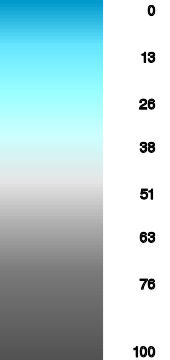
\includegraphics[angle=0,width=3.5cm,keepaspectratio='true']{figures/ramp-rasp-cloudpct.png} &
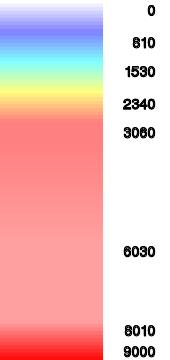
\includegraphics[angle=0,width=3.5cm,keepaspectratio='true']{figures/ramp-rasp-h.png} &
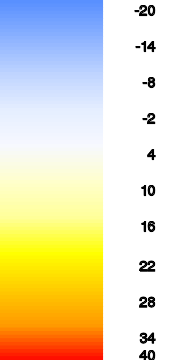
\includegraphics[angle=0,width=3.5cm,keepaspectratio='true']{figures/ramp-rasp-temperature.png} \\
\\
\emph{Vitesse verticale [m/s]} & \emph{Vitesse du vent [m/s]} & \\
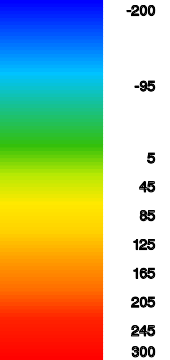
\includegraphics[angle=0,width=3.5cm,keepaspectratio='true']{figures/ramp-rasp-vertspeed.png} &
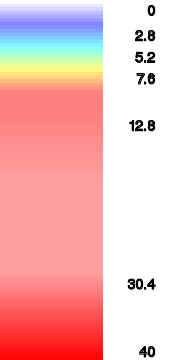
\includegraphics[angle=0,width=3.5cm,keepaspectratio='true']{figures/ramp-rasp-windspeed.png} & \\

\end{longtable}
\end{maxipage}

\section{pc\_met, Deutscher Wetterdienst}\label{sec:pcmet}

Le service météorologique allemand ``Deutscher Wetterdienst'' fournit plusieurs images météo utiles aux utilisateurs de \xc.
Pour les utiliser, vous avez besoin d'un compte (payant) incluant leur produit \emph{pc\_met}.

Notez que cette fonctionnalité nécessite et utilise une connexion Internet.
Cela peut être cher en fonction des caractéristiques de votre abonnement mobile.

Pour activer cette fonctionnalité, entrez vos identifiants \emph{pc\_met} dans le système de configuration d'\xc.
Il y a deux paires nom d'utilisateur/mot de passe~: le premier est pour les services web du DWD (\url{www.flugwetter.de}), le second est le mot de passe FTP (\url{ftp.pcmet.de}).

Au cours des vérifications pré-vol et pendant le vol, vous pouvez vérifier les prévisions météo et les données météo en temps réel dans le menu \menulabelr{\bmenug{Info}\blink\bmenug{Weather}} \bmenug{Info}.
Dans ``Surcouche'', vous pouvez choisir des couches pour la carte.
``pc\_met'' est une collection d'images en temps réel qui sont habituellement disponible sur le site web du DWD \url{www.flugwetter.de}.
